\chapter{Auswertung}
\label{ch:auswertung}





\section{Aufgabe 3: Qualitative Beobachtung der Umkehrung der Elektrolyse in einer Brennstoffzelle}

In dieser Aufgabe wird das Funktionsprinzip einer PEM-Brennstoffzelle untersucht, die die umgekehrte Reaktion der Elektrolyse nutzt. Der Versuch liefert qualitative Beobachtungen über die Umwandlung chemischer Energie in elektrische Energie.

\begin{enumerate}
    \item \textbf{Anode: Spaltung von Wasserstoff}\\
    Wasserstoff (H$_2$) wird an der Anode in Protonen (H$^+$) und Elektronen gespalten:
    \begin{equation*}
        2 \mathrm{H_2 \rightarrow 4 H^+ + 4 e^-} \quad (\text{\hyperref[eq:h2_anode]{Gleichung \ref*{eq:h2_anode}}})
    \end{equation*}
    Die Protonen passieren die protonenleitfähige Membran zur Kathode, während die Elektronen über einen externen Stromkreis fließen.
    
    \item \textbf{Kathode: Reaktion zu Wasser}\\
    An der Kathode reagieren Protonen, Elektronen und Sauerstoff zu Wasser:
    \begin{equation*}
        4 \mathrm{H^+ + 4 e^- + O_2 \rightarrow 2 H_2O} \quad (\text{\hyperref[eq:h2o_kathode]{Gleichung \ref*{eq:h2o_kathode}}})
    \end{equation*}
    Dabei entsteht Wasser, das als Kondensat sichtbar sein kann.

    \item \textbf{Gasverbrauch}\\
    Mit Beginn der Reaktion nimmt die Menge an Wasserstoff und Sauerstoff an den Elektroden ab, was die Umwandlung der chemischen Energie in elektrische Energie sichtbar macht.

    \item \textbf{Elektrischer Stromfluss}\\
    Ein angeschlossener Verbraucher kann die elektrische Energie abnehmen. Der Stromfluss zeigt die Nutzung der freiwerdenden Energie an.

    \item \textbf{Interpretation}\\
    Die Beobachtungen bestätigen die Umkehrung der Elektrolyse: Energie, die zuvor zur Zerlegung von Wasser benötigt wurde, wird nun durch die kontrollierte Reaktion von H$_2$ und O$_2$ freigesetzt und kann direkt als elektrische Energie genutzt werden.
\end{enumerate}

\section{Zusatz: Kupferoxidation an der Luft/unterm Föhn}
Wir wollen hier nun die Fehlerrechnung noch mal ein wenig vertiefen und eine weitere Fehlerquelle betracheten und ihren Einfluss untersuchen. Wir wollen schauen, wie viel Kupfer in der Zeit nach der Elektrolise und bis zum Wiegen Oxidieren.
Der Grund dafür ist, dass die zu wiegende Kathode nach der Elektrolyse kein konstantes Gewicht eingenommen hat, sondern das Gewicht über wenige Minuten um knapp $1mg$ anwuchst, ohne aufzuhören.
Die gestellte These hier ist, dass dies insbesondere durch den Einfluss des Föhns passiert, denn dieser hat die Kupferplatte erhitzt. Und bei Oxidationsvorgängen ist eine thermische Energiezufur equivalent zu einer Beschleunigung der Reaktion.
Die Platte hat sich dabei natürlcih nicht auf enorme Temperaturen erhitzt, aber es dürfte schon ausreichen, wenn die Oberfläche sich erhitzt, da sowieso nur an der Oberfläche die Oxidation stattfindet. In der Studie \cite{KupferStudie}
wurde mit Temperaturen im $60^\circ C$ gearbeitet. Für diese Untersuchung nehme ich die Werte als möglich an und als Basis der folgenden Untersuchung.

Wichtig ist hie rnatürlich zu erwähnen, dass die Rechnung kaum ernstzunehmen ist, die Werte und Überlegungen sind für sinnvolle Angaben kaum nutzbar und sollen erstmal die grundsetzliche Frage klären, ob die Oxidation an der Luft und das Fühnen einen signifikaten Einfluss haben könnten.

Dafür müssen wir einige Werte schätzen, dessen Messung leider nicht stattfund.
\begin{align}
    A_{Cu} &\approx (25 \pm 5)cm^2 \\
    t &\approx (300\pm100)s
\end{align}
Dabei ist $A_{Cu}$ die Kupferfläche, die Reagiert und $t$ die Zeit, in der die Reaktion stattfindet.

Wir leiten dabei graphisch die Massengewichstzunahme $\Delta m$ her. Dafür haben wir \hyperref[eq:stud_log]{Gleichung (\ref*{eq:stud_log})} in Python geplottet. Der Code fafür ist auf meinen GitHub \cite{githubPAP1}. 
Dabei sind vier \hyperref[fig:log_3]{Graphen \ref*{fig:log_3}} geplottet. Wir konzentrieren uns dabei auf die logarithmischskalierten Graphen und fabei auf den blauen (unterster) und den roten (obester) und suchen graphisch nach unserer Massenzunahme. 

Dabei kommen wir auf Werte von:
\begin{align}
    \Delta m_{min} &= (1,7 \pm 0,1)\frac{\mu g}{cm} \\
    \Delta m_{max} &= (2,4 \pm 0,14)\frac{\mu g}{cm}
\end{align}

Dabei haben wir daruf geachtet, nur im Bereich zu bleiben, der in der \hyperref[fig:stud_2]{Abbildung \ref*{fig:stud_2}} auch rot eingezeichnet ist zu bleiben.


\onecolumn
\begin{figure}
    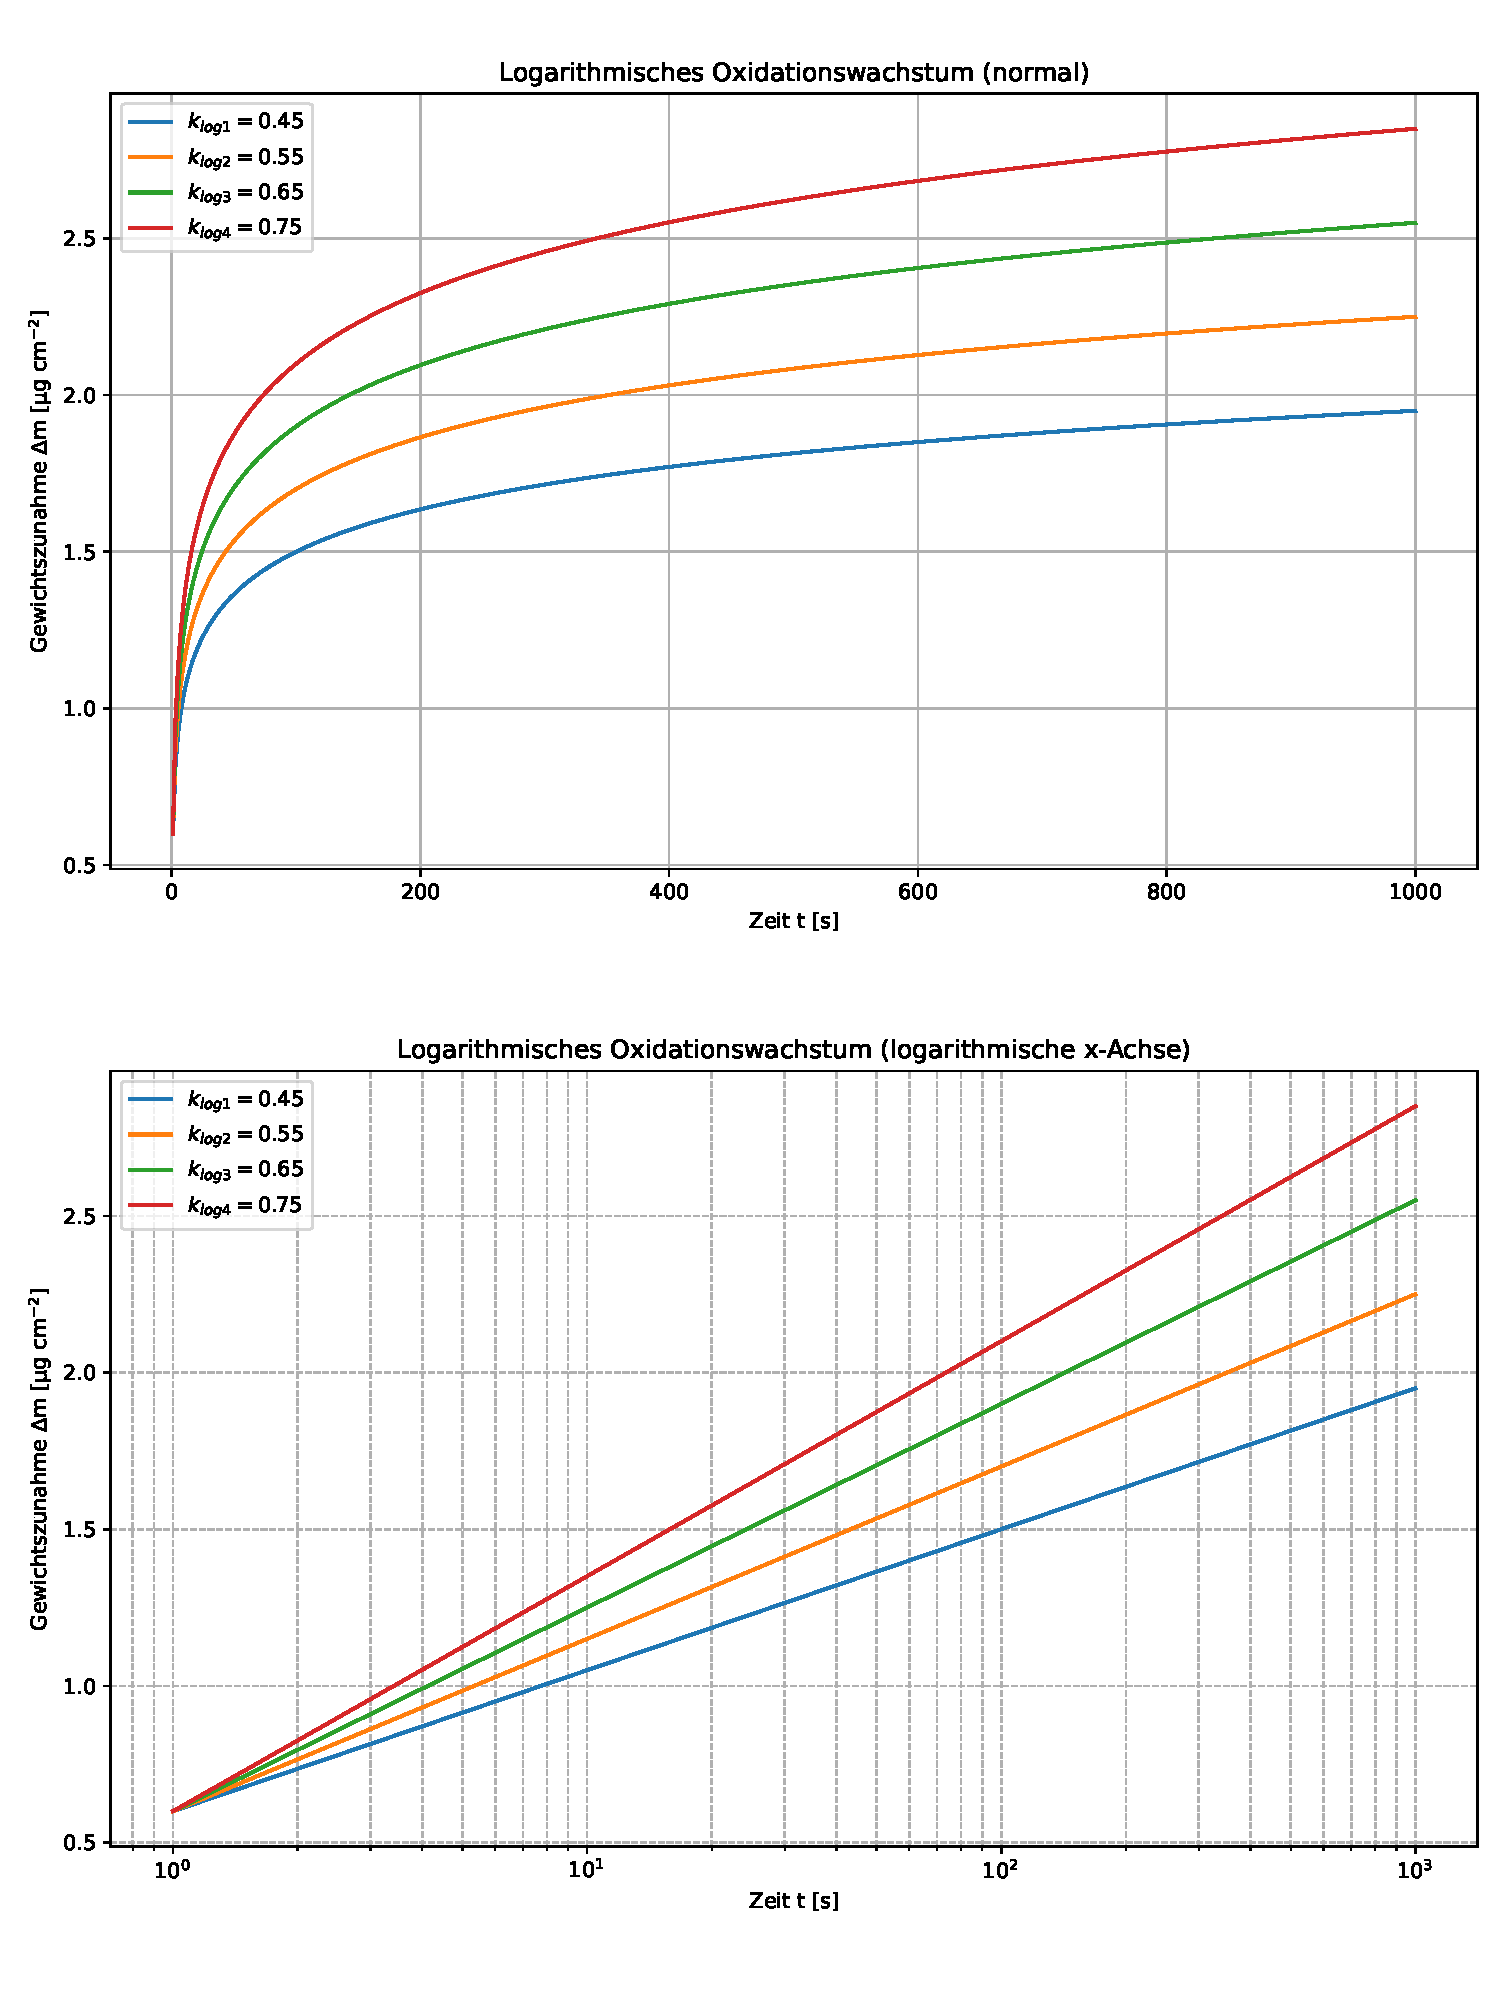
\includegraphics[width=\textwidth, page=1]{img/21/Plots_oxi.pdf}
    \caption{Entstandene Graphen aus der Gleichung, die in der Studie gegeben ist, mit verschiedenen $k_log$ konstanten.}
    \label{fig:log_3}
\end{figure}
\twocolumn